\documentclass{article}

\usepackage{polski}
\usepackage[utf8]{inputenc}

\usepackage{fancyhdr} % Required for custom headers
\usepackage{lastpage} % Required to determine the last page for the footer
\usepackage{extramarks} % Required for headers and footers
\usepackage[usenames,dvipsnames]{color} % Required for custom colors
\usepackage{graphicx} % Required to insert images
\usepackage{listings} % Required for insertion of code
\usepackage{courier} % Required for the courier font
\usepackage{lipsum} 
\usepackage{amsfonts}
\usepackage{amsthm}
\usepackage{hyperref}
\usepackage{tikz}
\usepackage{amsmath}
\usepackage{pdfpages}
\usepackage{mathtools}
\usepackage{enumitem}

\usepackage{amsthm}
\usepackage{epigraph}


\DeclareUnicodeCharacter{00A0}{ }

\makeatletter
\newenvironment{chapquote}[2][2em]
  {\setlength{\@tempdima}{#1}%
   \def\chapquote@author{#2}%
   \parshape 1 \@tempdima \dimexpr\textwidth-2\@tempdima\relax%
   \itshape}
  {\par\normalfont\hfill--\ \chapquote@author\hspace*{\@tempdima}\par\bigskip}
\makeatother

\newtheorem{thm}{Twierdzenie}
\newtheorem{remark}{Uwaga}
\newtheorem{lemat}{Lemat}
\newtheorem{wniosek}{Wniosek}
\newtheorem{definicja}{Definicja}
\newtheorem{ciekawostka}{Ciekawostka}
\newtheorem{przyklad}{Przykład}
\newtheorem{fakt}{Fakt}



\newenvironment{prooff}{\paragraph{Dowód:}}{\hfill$\square$}
\newenvironment{rozw}{\paragraph{Rozwiązanie:}}{\hfill}


% \usepackage{inconsolata} % very nice fixed-width font included with texlive-full
\usepackage[usenames,dvipsnames]{color} % more flexible names for syntax highlighting colors
\usepackage{listings}

\lstset{
basicstyle=\small\ttfamily, 
columns=fullflexible, % make sure to use fixed-width font, CM typewriter is NOT fixed width
numbers=left, 
numberstyle=\small\ttfamily\color{Gray},
stepnumber=1,              
numbersep=10pt, 
numberfirstline=true, 
numberblanklines=true, 
tabsize=4,
lineskip=-1.5pt,
extendedchars=true,
breaklines=true,        
keywordstyle=\color{Blue}\bfseries,
identifierstyle=, % using emph or index keywords
commentstyle=\sffamily\color{OliveGreen},
stringstyle=\color{Maroon},
showstringspaces=false,
showtabs=false,
upquote=false,
texcl=true, % interpet comments as LaTeX
    literate={á}{{\'a}}1 {ã}{{\~a}}1 {é}{{<}}1,
inputencoding=utf8
}

\lstdefinelanguage{julia}
{
  keywordsprefix=\@,
  morekeywords={
    exit,whos,edit,load,is,isa,isequal,typeof,tuple,ntuple,uid,hash,finalizer,convert,promote,
    subtype,typemin,typemax,realmin,realmax,sizeof,eps,promote_type,method_exists,applicable,
    invoke,dlopen,dlsym,system,error,throw,assert,new,Inf,Nan,pi,im,begin,while,for,in,return,
    break,continue,macro,quote,let,if,elseif,else,try,catch,end,bitstype,ccall,do,using,module,
    import,export,importall,baremodule,immutable,local,global,const,Bool,Int,Int8,Int16,Int32,
    Int64,Uint,Uint8,Uint16,Uint32,Uint64,Float32,Float64,Complex64,Complex128,Any,Nothing,None,
    function,type,typealias,abstract
  },
  sensitive=true,
  morecomment=[l]{\#},
  morestring=[b]',
  morestring=[b]" 
}

% Margins
\topmargin=-0.45in
\evensidemargin=0in
\oddsidemargin=0in
\textwidth=6.0in
\textheight=9.0in
\headsep=0.25in

\linespread{1.1} % Line spacing

% Set up the header and footer
\pagestyle{fancy}
\lhead{\hmwkAuthorName} % Top left header
\rhead{\firstxmark} % Top right header
\lfoot{\lastxmark} % Bottom left footer
\cfoot{} % Bottom center footer
\renewcommand\headrulewidth{0.4pt} % Size of the header rule
\renewcommand\footrulewidth{0.4pt} % Size of the footer rule

\setlength\parindent{0pt} % Removes all indentation from paragraphs
%----------------------------------------------------------------------------------------
%	DOCUMENT STRUCTURE COMMANDS
%	Skip this unless you know what you're doing
%----------------------------------------------------------------------------------------

% Header and footer for when a page split occurs within a problem environment
\newcommand{\enterProblemHeader}[1]{
\nobreak\extramarks{#1}{#1 continued on next page\ldots}\nobreak
\nobreak\extramarks{#1 (continued)}{#1 continued on next page\ldots}\nobreak
}

% Header and footer for when a page split occurs between problem environments
\newcommand{\exitProblemHeader}[1]{
\nobreak\extramarks{#1 (continued)}{#1 continued on next page\ldots}\nobreak
\nobreak\extramarks{#1}{}\nobreak
}

\setcounter{secnumdepth}{0} % Removes default section numbers
\newcounter{homeworkProblemCounter} % Creates a counter to keep track of the number of problems

\newcommand{\homeworkProblemName}{}
\newenvironment{homeworkProblem}[1][Zadanie \arabic{homeworkProblemCounter}]{ % Makes a new environment called homeworkProblem which takes 1 argument (custom name) but the default is "Problem #"
\stepcounter{homeworkProblemCounter} % Increase counter for number of problems
\renewcommand{\homeworkProblemName}{#1} % Assign \homeworkProblemName the name of the problem
\section{\homeworkProblemName} % Make a section in the document with the custom problem count
\enterProblemHeader{\homeworkProblemName} % Header and footer within the environment
}{
\exitProblemHeader{\homeworkProblemName} % Header and footer after the environment
}

\newcommand{\problemAnswer}[1]{ % Defines the problem answer command with the content as the only argument
\noindent\framebox[\columnwidth][c]{\begin{minipage}{0.98\columnwidth}#1\end{minipage}} % Makes the box around the problem answer and puts the content inside
}

\newcommand{\homeworkSectionName}{}
\newenvironment{homeworkSection}[1]{ % New environment for sections within homework problems, takes 1 argument - the name of the section
\renewcommand{\homeworkSectionName}{#1} % Assign \homeworkSectionName to the name of the section from the environment argument
\subsection{\homeworkSectionName} % Make a subsection with the custom name of the subsection
\enterProblemHeader{\homeworkProblemName\ [\homeworkSectionName]} % Header and footer within the environment
}{
\enterProblemHeader{\homeworkProblemName} % Header and footer after the environment
}

\usepackage{listings} % Required for inserting code snippets
\usepackage[usenames,dvipsnames]{color} % Required for specifying custom colors and referring to colors by name

\definecolor{DarkGreen}{rgb}{0.0,0.4,0.0} % Comment color
\definecolor{highlight}{RGB}{255,251,204} % Code highlight color

% Create a command to cleanly insert a snippet with the style above anywhere in the document
\newcommand{\insertcode}[2]{\begin{itemize}\item[]\lstinputlisting[caption=#2,label=#1,style=Style1]{#1}\end{itemize}} % The first argument is the script location/filename and the second is a caption for the listing

%----------------------------------------------------------------------------------------
%	NAME AND CLASS SECTION
%----------------------------------------------------------------------------------------

\newcommand{\hmwkTitle}{Problem biesiadujących filozofów} % Assignment title
\newcommand{\hmwkDueDate}{} % Due date
\newcommand{\hmwkClass}{Systemy operacyjne} % Course/class
\newcommand{\hmwkClassTime}{} % Class/lecture time
\newcommand{\hmwkClassInstructor}{} % Teacher/lecturer
\newcommand{\hmwkAuthorName}{Jan Góra - obowiązkowe zadanie z systemów operacyjnych} % Your name

%----------------------------------------------------------------------------------------

\begin{document}

\title{Problem biesiadujących filozofów}
\date{\today}
\author{Jan Góra}

\maketitle

%%%%%%%%%%%%%%%%%%%%%%%%%%%%%%%%%%%%%%%%%%%%%%%%%%%%%%%%%%%%%%%%%%%%%%%%%%%

\subsection*{Treść zadania}

\begin{center}
\begin{tikzpicture}
\node [draw={black}, fill=black!10, very thick, rectangle, rounded corners, inner sep=12pt, inner ysep=12pt] (box){%
    \begin{minipage}{.9\textwidth}

Przy okrągłym stole biesiaduje $N$ filozofów i każdy wykonuje jedną z dwóch czynności – albo je, albo rozmyśla. Przed każdym z nich znajduje się talerz, a pomiędzy każdą sąsiadującą parą filozofów leży pałeczka, a więc każdy ma przy sobie dwie sztuki – po swojej lewej i prawej stronie. Ponieważ jedzenie potrawy jest trudne przy użyciu jednej pałeczki, zakłada się, że każdy filozof korzysta z dwóch. Dodatkowo nie ma możliwości skorzystania z pałeczki, która nie znajduje się bezpośrednio przed daną osobą. Liczba dostępnych dań ograniczona jest przez liczbę $M$.
\bigskip

Uogólnić problem na problem synchronizacji procesów systemowych.

    \end{minipage}
};
\node[fill={black}, text=white, rounded corners, right=10pt] at (box.north west) {Problem oraz treść zadania};
\end{tikzpicture}
\end{center}

Podczas rozwiązywania zadania występić mogą następujące problemy:

\begin{itemize}
\item Każdy z nich zabierze lewą pałeczkę i będzie czekał na prawą (lub na odwrót) - \textbf{zakleszczenie}
\item Niezależnie od zakleszczenia, dojść może do bardzo zróżnicowanego dostępu do posiłków - \textbf{zagłodzenie}
\end{itemize}

\subsection*{Rozwiązanie}

Powyższy problem bardzo łatwo uogólnić na problem synchronizacji procesów systemowych. W rozwiązaniu, poprzez biesiadującego filozofa będziemy rozumieć proces, a dostęp do pałeczek oraz dostępnych dań będziemy rozumieć jako sekcję krytyczną, tzn. fragment programu odpowiadający za korzystanie z zasobów dzielonych.  Do zarządzenia wyżej wymienionej sekcją użyte zostały semafory.\bigskip

Jednym z rozwiązań problemu ucztujących filozów, a dokładniej problemu \textbf{zakleszczenia}, jest ograniczenie liczby dostępnych talerzy, przy warunku, że filozof bez talerza nie może podnieść pałeczki ze stołu. Łatwo zauważyć, że przy ograniczeniu talerzy poprzez liczbę $N-1$, przynajmniej jeden z filozofów podniesie obie pałeczki, w następstwie czego przynajmniej jeden filozof zje w tym czasie jedną potrawę. Na mocy indukcji, z obserwacji tej wprost wynika, że wszystkie posiłki zostaną zjedzone oraz, że nie nastąpi zakleszczenie cykilczne, ponieważ aby owe zakleszczenie, przy tak sformułowanym zadaniu wystąpiło, wszystkie procesy muszą się wzajemnie ,,zakleszczyć''. 

\bigskip

Obok talerzy i pałeczek, kolejnym zasobem dzielonym jest liczba dostępnych dań, w wyniku czego podniesienie obu pałeczek nie jest warunkiem wystarczającym do zjedzenia posiłku -- dany proces musi jeszcze wygrać ,,wyścig'' po potrawę, co w teorii może nigdy nie nastąpić. 

Rozwiązanie problemu \textbf{zagłodzenia} jest bardziej problematyczne. W praktyce niekoniecznie będziemy chcieli, aby każdy z procesów otrzymał równy dostęp do dzielonych zasobów oraz, aby każdy z procesów odpytywał o zasób z tą samą częstotliwością. Jako, że filozof oprócz jedzenia również rozmyśla, rozmyślanie blokuje go przed zjedzeniem posiłku na pewien czas. Zauważmy, że im szerszy przedział długości oczekiwania względem liczby wszystkich filozofów, tym dostęp do dzielonych zasobów będzie łatwiejszy, w wyniku czego dostęp do pałeczek będzie niemal równoznaczny ze zjedzeniem posiłku, a dostęp do talerza skutkować będzie dostępem do obu pałeczek. W dołączonym rozwiązaniu czas oczekiwania, w mikrosekundach, wybierany jest losowo z przedziału $[0,N)$, co w znaczeniu przenośnym oznacza: ,,wyliczanie aż do znudzenia kolejnych filozofów''. Idea pomysłu jest taka, aby nie pozbywać się zupełnie rywalizacji o zasoby, ale jednocześnie rywalizację tę znacząco zmniejszyć.


\bigskip

Rozwiązanie umieszczone jest w katalogu \emph{Filozofowie} dołączonym do sprawozdania.

Pałeczkom odpowiada tablica semaforów (\textbf{stick[$N$]}) o buforach rozmiaru $1$.

Talerzom odpowiada semafor (\textbf{plates}) o buforze rozmiaru $N-1$.

Pozostałej liczbie dostępnych posiłków odpoawiada zmienna typu \emph{int} (\textbf{dishes\_left}) oraz semafor o buforze (\textbf{eating}) rozmiaru $1$ kontrolującym dostęp do tej zmiennej.

Każdy proces (filozof) jest ponumerowany od $0$ do ${N-1}$, a swoje działanie kończy w przypadku gdy zmienna \textbf{dishes\_left} jest równa 0. 

Program kończy swoje działanie, kiedy nie ma żadnych aktywnych procesów pochodnych.

Przykładowy wynik uruchomienia programu, który możemy zaobserwować w grafice załączonej poniżej, działa zgodnie z oczekiwaniami, tj. procesy o najdłuższym okresie ,,rozmyślania'' zużyły najmniej zasobów.

\begin{figure}[h!]
\centering
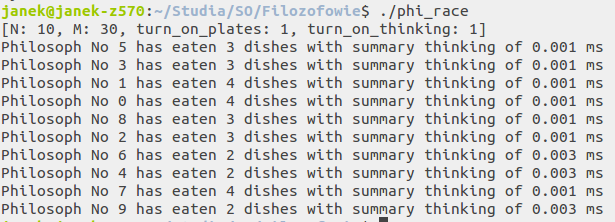
\includegraphics[scale=0.5]{example}
\end{figure} 


\subsection{Testy}
Program testowany był w przeróżnych konfiguracjach. Udawało mi się osiągnąć efekt zakleszczenia przy danych \textbf{N = 10}, \textbf{M = 10000000}, \textbf{turn\_plates\_on = false} oraz \textbf{turn\_thinking\_on = false}. Jednak, co jest bardzo interesujące, po zrestartowaniu komputera nie udaje mi się odtworzyć tego efektu. W przeprowadzonych testach, zgodnie z oczekiwaniami, liczba dań zjedzonych przez filozofów za każdym razem sumowała się do liczby M, co dowodzi tego, że brak jest wycieków dzielonych zasobów -- w danym czasie dostęp do nich miał maksymalnie jeden proces. Dla kontrastu bez używania semafora \textbf{eating} liczba ta prawie nigdy sumowała się prawidłowo.
\bigskip

Przy ustawionych zmiennych: \textbf{turn\_plates\_on = false} i \textbf{turn\_thinking\_on = false}, przy zbliżonym stosunku $M$ do $N$ podział zasobów jest bardzo różny, a wraz ze wzrostem ilości dostępnych zasobów, podział ten stawał się bardziej równomierny. 

\begin{figure}[h!]
\centering
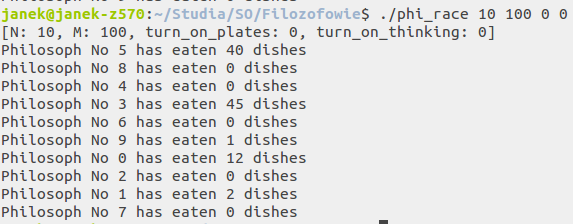
\includegraphics[scale=0.4]{test_10_100_0_0.png}
\end{figure} 
\begin{figure}[h!]
\centering
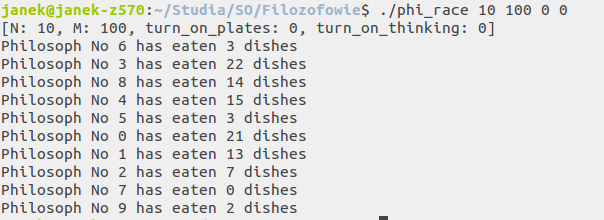
\includegraphics[scale=0.4]{test2_10_100_0_0.png}
\end{figure} 
\begin{figure}[h!]
\centering
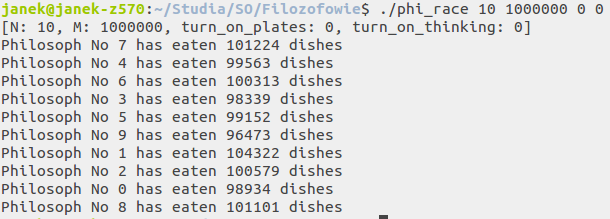
\includegraphics[scale=0.4]{test2_10_1000000_0_0.png}
\end{figure} 

\newpage

Włączenie semafora przydzielającego talerze przyczyniło się do  prawie całkowitego wyelimowania całkowitego zagłodzenia, jednak nie poprawiło to równomiernego przydziału zasobów. Natomiast wprowadzenie oczekiwania o losowej długości (w mikrosekundach, z przedziału $[0, N)$) poskutkowało niemal idealnie równomiernym podziałem zasobów. Dzieje się tak, ponieważ rywalizacja o zasób jedzenia jest znacząco mniejsza, co skutkuje mniejszą losowością wyników. W poprzednich przykładach, o dostęp do tego semafora mogło walczyć nawet $\frac{1}{2}N$ procesów. Najlepsze rezultaty uzyskuje się przy jednoczesnym aktywowaniu obu semaforów. 

\begin{figure}[h!]
\centering
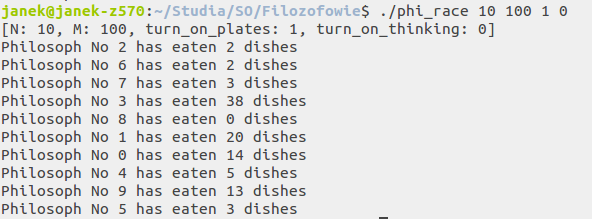
\includegraphics[scale=0.4]{test_10_100_1_0.png}
\end{figure} 

\begin{figure}[h!]
\centering
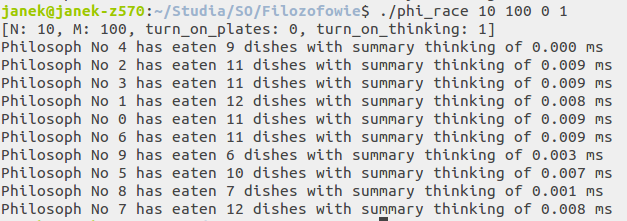
\includegraphics[scale=0.4]{test_10_100_0_1.png}
\end{figure} 

\begin{figure}[h!]
\centering
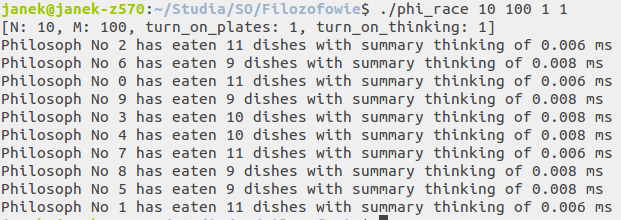
\includegraphics[scale=0.4]{test_10_100_1_1.png}
\end{figure} 

\newpage
Podczas gdy \textbf{$N = 10^3$} (liczba procesów) i \textbf{$M = 10^7$} (liczba zasobów), oczekiwać by można, że program będzie wykonywać się bardzo długo. Naiwna implementacja synchronizacji procesów mogłaby być nawet rzędu \textbf{$O(N*M) = O(10^{10})$}, aczkolwiek jak zostało pokazane na przykładzie, czas uruchomienia programu był zaskakująco niski -- \textbf{19.232s}!! 

Podział zasobów nie tylko jest równomierny dla małych danych, ale również dla bardzo dużych. Co można zobaczyć w kolejnym przykładzie. Interesującą obserwacją jest to, że pod koniec standardowego wyjścia pojawia się dosłownie parę procesów o niskim zużyciu zasobów (np. No 895 = 17 i No 890 = 90), czego nie zaobserwowałem przeglądając wyniki w głąb. 

\begin{figure}[h!]
\centering
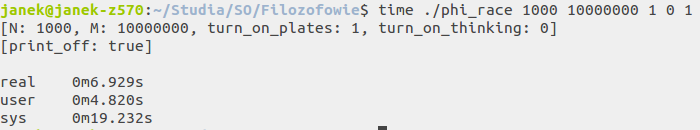
\includegraphics[scale=0.4]{test_time2.png}
\end{figure} 

\begin{figure}[h!]
\centering
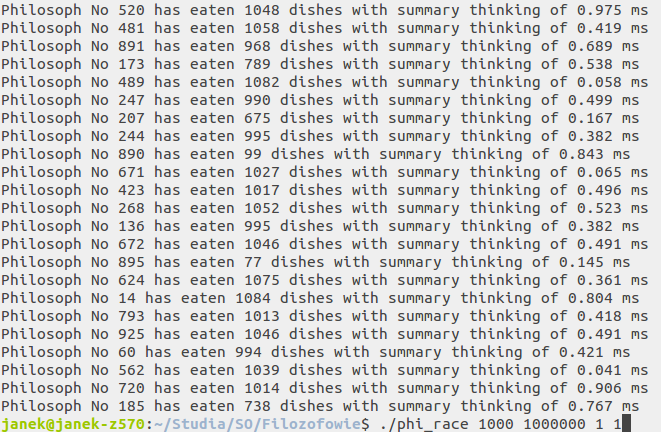
\includegraphics[scale=0.4]{test_bigtest.png}
\end{figure} 

\subsection*{Uwagi techniczne}

Do rozwiązania załączony został plik \textbf{Makefile} stworzony tak, aby po wywołaniu polecenia \textbf{make} otrzymać pliki binarne, a po wywołaniu polecenia \textbf{make clean} usunąć je. W przeciwnym wypadku program powinien zostać skompilowany użwyjąc komendy: \textbf{\$ gcc -std=gnu99 -pthread phi\_race.c -o phi\_race -lrt}. Program wykonywać można z argumentami, którego wywołanie wygląda następująco \textbf{\$ ./phi\_race ?N ?M ?turn\_plates\_on ?turn\_thinking\_on ?print\_off}, gdzie \emph{?N} i \emph{?M} jest typu \emph{int}, a reszta argumentów przyjmuje wartości 0 lub 1



\end{document}